\chapter{Colouring}
\lecture{3}{21/10}

Many algorithms are \emph{recursive}, at each level of recursion we
\begin{description}
    \item[divide] the problem into a number of subproblems;
    \item[conquer] the subproblems by solving them recursively, or
        if the subproblem is small enough trivially; then
    \item[combine] the solutions for the subproblems into a solution
        for the origin problem.
\end{description}

\begin{example}
    \texttt{MergeSort} and \texttt{QuickSort} are examples
    of divide-and-conquer algorithms.
\end{example}

\begin{definition}[Colouring]
    A \textbf{colouring} is an assignment of colours to the vertices of a graph
    such that no two adjacent vertices get the same colour.
\end{definition}

A colouring using at most $k$ colours is a \textbf{$k$-colouring}.
The \textbf{chromatic number} $\chi_G$ of a graph $G$
is the smallest integer $k$ for which $G$ has a $k$-colouring.

\begin{problem}[Colouring]
    Give a graph $G$, determine $\chi_G$.
\end{problem}

The colouring problem is NP-hard (definition of this to follow)
and as such no polynomial-time algorithm is known.

There are a number of ways to deal with NP-hard problems, for example:
\begin{enumerate}
    \item heuristics;
    \item approximation algorithms;
    \item exact algorithms;
    \item parameterised algorithms; and
    \item algorithms for restricted inputs.
\end{enumerate}

We are going to focus on algorithms for restricted inputs.
That is, we will exploit the structure of the input with the
aim of developing a faster algorithm.
We can justify this because
\begin{enumerate}
    \item in practise, problem inputs have a structure; and
    \item by focussing on the input structure we can better understand
        what structure makes a problem computationally hard.
\end{enumerate}

\begin{definition}[Graph operations]
    Let $G_1 = (V_1, E_1)$ and $G_2 = (V_2, E_2)$ be two vertex-disjoint graphs.
    Then
    \begin{enumerate}
        \item ( \textbf{disjoint union} )
            \[
                G_1 + G_2 = (V_1 \cup V_2, E_1 \cup E_2);
            \]

        \item ( \textbf{join} )
            \[
                G_1 \times G_2 = (G_1 \cup G_2, E_1 \cup E_2 \cup E^\star)
            \]
            where $E^\star$ is the set of all edges
            between vertices in $V_1$ and vertices in $V_2$.
    \end{enumerate}
\end{definition}

\begin{definition}[Cograph]
    Let $G_1$ and $G_2$ be cographs.
    A graph $G$ is a \textbf{cograph} if and only if $G$ can be created
    by the following rules:
    \begin{enumerate}
        \item $K_1$ is a cograph;
        \item $G_1 + G_2$ is a cograph; and
        \item $G_1 \times G_2$ is a cograph.
    \end{enumerate}
\end{definition}

\begin{definition}[Induced subgraph]
    Let $G$ be a graph.
    We say that $G' \subset G$ is an
    \textbf{induced subgraph} of
    $G$ if $G$ can be modified to $G'$ via vertex deletions.
\end{definition}

\begin{definition}[$P_4$]
    We denote the path on $4$ vertices as $P_4$.
\end{definition}

\begin{figure}
    \centering
    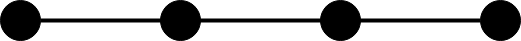
\includegraphics[width=0.8\linewidth]{images/p4.png}
    \caption{$P_4$ graph.}
    \label{fig:p4}
\end{figure}

If a graph $P_4$ is not an induced subgraph of a graph $G$, we say that it is \textbf{$P_4$-free}.

\begin{theorem}[]
    A graph is a cograph if and only if it is $P_4$-free.
\end{theorem}

\begin{definition}[Cotree]
    A cotree $T$ is a tree in which we label internal nodes $+$ or $\times$. $T$ defines a cograph $G$ where the leaves of $T$ correspond to $V(G)$. 
    Each subtree $T' \subset T$ corresponds to an inducted subgraph $G' \subset G$ defined by the set of leaves descending from it. 
    We have the following properties:
    \begin{enumerate}
        \item a subtree consisting of a single node corresponds to the induced subgraph of one vertex (clearly);
        \item a subtree rooted with $T$ corresponds to the union of the subgraphs defined by the children; and
        \item a subtree rooted with $x$ corresponds to the join of the subgraphs correponding to the leaves.
    \end{enumerate}
\end{definition}

\begin{proposition}[]
    For a cograph $G$ with corresponding cotree $T$, then
    \[ \chi_G = \max_{v \in V(G)}\{\operatorname{count}{(\operatorname{children{(v)}})}\}. \] 
\end{proposition}

% todo read up on this, it is very interesting.
